\chapter[Obtención y Tratamiento de los datos]{Obtención y Tratamiento de los datos}
\label{cp:obtencion}

Antes de profundizar en el diseño y entrenamiento de las redes neuronales, es fundamental conocer la naturaleza de los datos utilizados en 
este trabajo. En el ámbito de la teledetección aplicada a la \acrshort{ia}, el éxito de un modelo depende en gran medida de la calidad, formato
y coherencia de los datos con los que se nutre al modelo. Por ello, en este capítulo se definen los datos con los que estamos trabajando, bajo
qué marco de referencia geográfico se rigen y las transformaciones necesarias para convertirlos en datos útiles para nuestros modelos de 
aprendizaje profundo.


A lo largo del capítulo, se detallará el proceso de obtención de las imágenes multiespectrales y cartografía con las coberturas del suelo, pasando
por la concordancia de sus coordenadas, hasta la fragmentación física del territorio en más de un millón de parches matriciales de entrada y salida.
Este proceso garantiza que cada píxel de las coordenadas de las bandas espectrales coincida con las etiquetas de uso, a nivel de píxel, construyendo
así una base de datos dual (Sentinel-2 - CORINE Land Cover España).  

\section{Adquisición de fuentes masivas: \acrlong{gee} y \acrshort{cnig}}
\label{data_source}

El primer reto del proyecto consistió en la extracción y descarga de las fuentes de datos geoespaciales a gran escala. Para ello se recurrió a
la plataforma \acrfull{gee} para las imágenes de satélite y al servidor oficial de \acrshort{corine} Land Cover España para la cartografía base.


\subsection{Extracción de los espectros mediante \acrshort{gee}}

Para la obtención de la información espectral se utilizó la plataforma \acrshort{gee}, empleando la API de Javascript para descargar los datos
de forma automática. Para agilizar los procesos se separó la descarga en 6 parches distintos, cuatro en la zona central de España expandiendose hasta
Valencia, uno en Galicia, para representar la costa gallega, y otro en Andalucía. Las coordenadas de cada parche son las siguientes, bajo el 
sistema de referencia global WGS 84 (\acrshort{epsg}:4326), la cual usa grados para representar las coordenadas de la Tierra:
\begin{itemize}
    \item Cuadrante Central Noroeste (NW): Delimitado entre las longitudes -6.0 y -3.0 y latitudes 40.5 y 43.0
    \item Cuadrante Central Noreste (NE): Delimitado entre las longitudes -3.0 y -0.5 y latitudes 40.5 y 42.5
    \item Cuadrante Central Suroeste (SW): Delimitado entre las longitudes -6.0 y -3.0 y latitudes 38.0 y 40.5
    \item Cuadrante Central Sureste (SE): Delimitado entre las longitudes -3.0 y -0.5 y latitudes 38.0 y 40.5
    \item Cuadrante Gallego: Delimitado entre las longitudes -9.3 y -7.5 y latitudes 42.2 y 43.8
    \item Cuadrante Andaluz: Delimitado entre las longitudes -6.5 y -1.6 y latitudes 36.0 y 37.2
\end{itemize}

Estas coordenadas generan los siguientes macro-parches para nuestro proyecto, como se puede ver en la Figura \ref{fig:parches}:

\begin{figure}[!htpb]
    \centering
    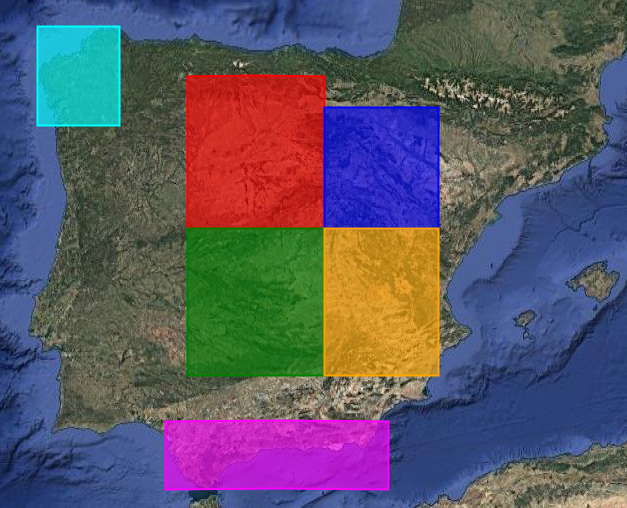
\includegraphics[width=0.5\linewidth]{Img/Theme/macroparches.png}
    \caption[Macro-parches España]{Representación de los 6 macro-parches generados mediante el motor de \acrshort{gee} \cite{googleearthengine.com}}
    \label{fig:parches}
\end{figure}


Para cada una de estas regiones, se realizó una consulta a los datos extraídos por el satélite Sentinel-2A, el cual ofrece los valores de reflectancia
en la superficie corregidos atmosféricamente \cite{sentinel2}. La búsqueda se acotó entre el 1 de junio y el 30 de septiembre de 2018, con el fin 
de conseguir una coherencia con los datos extraídos de \acrshort{clc} España 2018. Se aplicó un filtro por el cual se ignoraron fotos con más de 
un 10\% de nubes. También se aplicó un filtro por el cual se toma la mediana de cada uno de los píxeles para evitar nubes puntuales, o cualquier
cosa que pueda distorsionar la señal. Finalmente se aplicó un filtro con el cual cualquier imagen fuera de territorio español fuera eliminada, principalmente las relativas al mar.


Una vez se tienen ya todas las imágenes con el menor número de imperfecciones posibles, se genera un mosaico con todas las imágenes del satélite
superpuestas para crear cada uno de los macroparches. De este mosaico se seleccionan únicamente las bandas de 10 metro de resolución por píxel, 
B02 (espectro azul), B03 (espectro verde), B04 (espectro rojo) y B08 (espectro \acrshort{nir}), con el fin de no saturar la memoria de los 
equipos con los que trabajamos. Estas imágenes con el fin de mantener una coherencia se descargaron bajo el marco de referencia \acrshort{epsg}:25830
con el fin de que fuera más sencillo de procesar después y sincronizar con la base de datos de \acrshort{clc} España 2018. Una vez aplicados
todos los filtros y seleccionadas las bandas deseadas, los mosaicos se exportan a Google Drive en formato GeoTIFF.


\subsubsection{Visualización de los parches mediante QGIS}

